\documentclass[11pt,a4paper]{article}

\usepackage[margin=2.4cm]{geometry}
\usepackage[T1]{fontenc}
\usepackage[utf8]{inputenc}
\usepackage{amsmath}
\usepackage{mathpazo}
\usepackage{microtype}
\usepackage{booktabs}
\usepackage{graphicx}
\usepackage{xcolor}
\usepackage{titlesec}
\usepackage{enumitem}
\usepackage[hidelinks]{hyperref}
\usepackage{caption}

\definecolor{rule}{HTML}{BBBBBB}
\captionsetup{font=small,labelfont=bf,skip=4pt}
\setlist{nosep,leftmargin=1.4em}
\titleformat{\section}{\large\bfseries}{\thesection}{0.7em}{}
\titlespacing{\section}{0pt}{1.5ex plus .2ex}{0.7ex}
\setlength{\parskip}{0.55ex}
\setlength{\parindent}{0pt}
\renewcommand{\arraystretch}{1.15}
\newcommand{\code}[1]{\texttt{\small #1}}

\hyphenpenalty=10000
\exhyphenpenalty=10000
\tolerance=2000
\emergencystretch=3em
\sloppy

\title{\vspace{-1.5cm}\textbf{Reactions to the Gillette ``We Believe'' Advertisement\\
on r/MensLib and r/MensRights}\\[0.3em]
\large Findings}
\date{\vspace{-0.4em}\normalsize 16 October 2026\vspace{-0.6em}}
\author{}

\begin{document}
\maketitle
\vspace{-1.1cm}

\noindent\textcolor{rule}{\rule{\linewidth}{0.4pt}}
\vspace{0.8em}

Measures, sample construction, inference and validation are documented separately in
\emph{Methodology, Statistics and Replication Materials}. This document reports what was found.
Throughout, \emph{tone} is the affective valence of a comment's text and \emph{stance} is the
position it takes on the advertisement; the two come apart, and most of what follows depends on
the distinction.

\section{The communities took opposite positions on the ad}

Among comments that take a position, \textbf{86.4\,\% of r/MensRights is critical of the
advertisement against 12.9\,\% of r/MensLib, which is 71.8\,\% supportive.} The gap in critical
share is $-73.7$ points (95\,\% CI $-78.3$ to $-69.6$).

\begin{figure}[h]
\centering
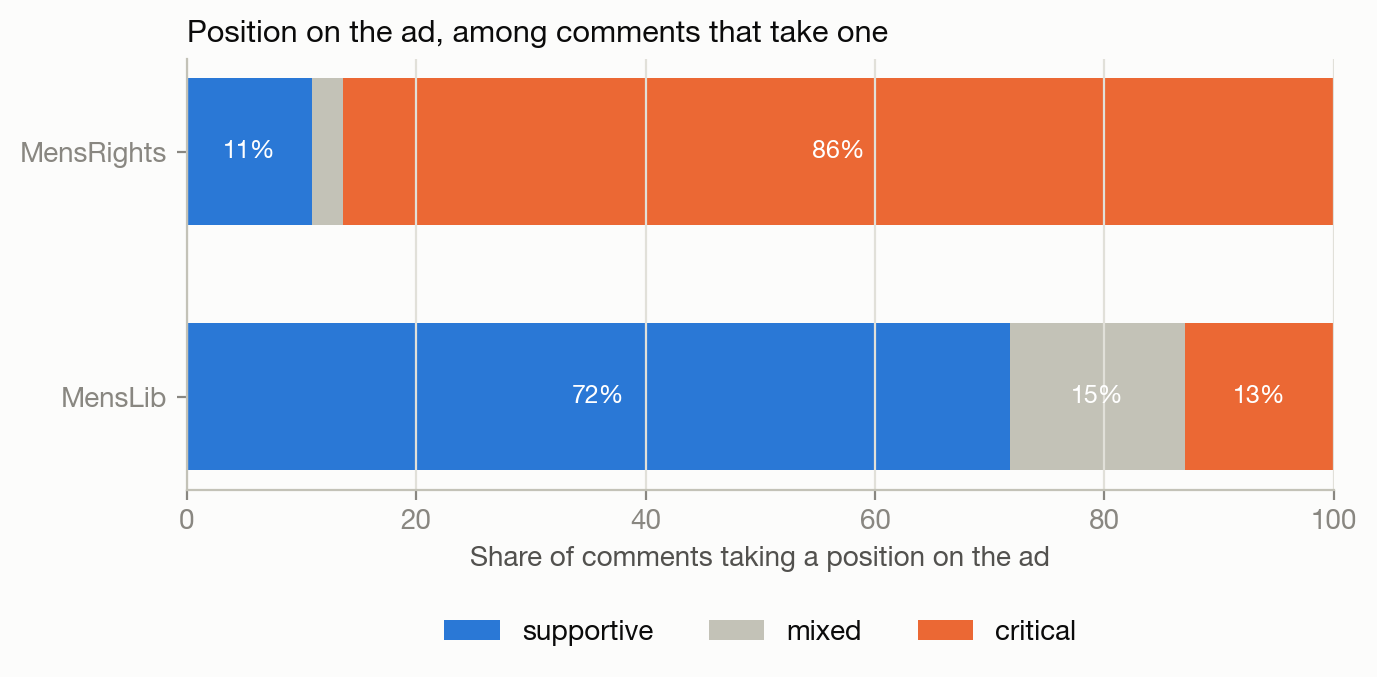
\includegraphics[width=0.92\linewidth]{figs/stance_composition.png}
\caption{Position on the advertisement, among the 6{,}552 comments that take one}
\end{figure}

Both communities engage at a similar rate: 38.2\,\% of r/MensLib comments and 42.0\,\% of
r/MensRights comments take a position at all. The difference lies in what they said, not in how
much they cared.

The result holds from $-70$ to $-75$ points across every specification tried, and it survives the
moderation problem described in \S4: assuming every removed r/MensLib comment was critical and
every removed r/MensRights comment was supportive, the gap still runs from $-50$ to $-77$ points.
Adjusting for comment length, reply depth and period, the odds that a positioned comment is
critical are \textbf{34.9 times higher} in r/MensRights (95\,\% CI 24.4 to 49.9).

\section{Resentment, identity threat, zero-sum thinking and hostility}

All four constructs are higher in r/MensRights, with zero-sum thinking showing the largest relative
gap and resentment the largest absolute one.

\begin{table}[h]
\centering\small
\caption{Construct ratings, 0--3, where 0 is absent and 3 strong and central}
\begin{tabular}{lcccc}
\toprule
& Resentment & Identity threat & Zero-sum & Hostility \\
\midrule
r/MensLib, mean          & 0.333 & 0.340 & 0.057 & 0.122 \\
r/MensRights, mean       & 0.908 & 0.747 & 0.451 & 0.416 \\
Clearly present ($\geq 2$), r/MensLib    & 5.2\,\%  & 10.4\,\% & 0.5\,\%  & 1.5\,\% \\
Clearly present ($\geq 2$), r/MensRights & 29.8\,\% & 23.6\,\% & 11.2\,\% & 10.1\,\% \\
Difference [95\,\% CI]   & $-0.575$ & $-0.407$ & $-0.394$ & $-0.294$ \\
                         & \footnotesize $[-0.66, -0.48]$ & \footnotesize $[-0.57, -0.24]$ & \footnotesize $[-0.44, -0.34]$ & \footnotesize $[-0.33, -0.27]$ \\
Cliff's $\delta$         & $-0.292$ & $-0.192$ & $-0.276$ & $-0.178$ \\
\bottomrule
\end{tabular}
\end{table}

Zero-sum thinking is roughly seven times more present in r/MensRights and close to absent in
r/MensLib, where only 0.5\,\% of comments rate it clearly present. Resentment is the largest in
absolute terms: nearly a third of r/MensRights comments carry a clear sense that men are being
wronged.

\begin{figure}[h]
\centering
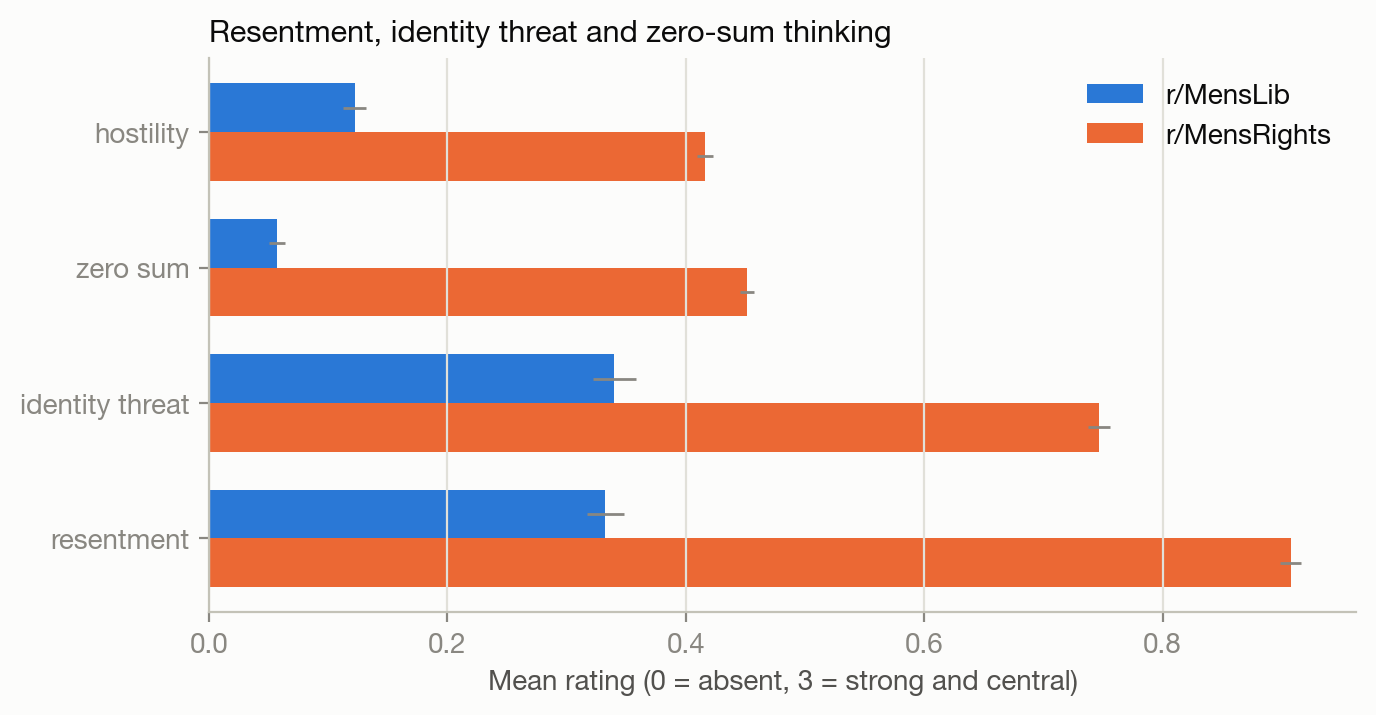
\includegraphics[width=0.88\linewidth]{figs/constructs.png}
\caption{Mean construct ratings; bars show bootstrap standard errors}
\end{figure}

\subsection*{The constructs belong to the position, not the community}

Splitting by coded stance rather than by subreddit changes the picture, and this is the more
interesting result.

\begin{table}[h]
\centering\small
\caption{Construct means by coded stance, pooling both subreddits}
\begin{tabular}{lrcccc}
\toprule
Stance & $n$ & Resentment & Identity threat & Zero-sum & Hostility \\
\midrule
Critical         & 5{,}284 & 1.830 & 1.610 & 0.982 & 0.698 \\
Mixed            & 242     & 0.946 & 1.054 & 0.306 & 0.095 \\
Supportive       & 1{,}026 & 0.432 & 0.440 & 0.066 & 0.317 \\
Not about the ad & 9{,}172 & 0.344 & 0.216 & 0.135 & 0.231 \\
\bottomrule
\end{tabular}
\end{table}

Comments critical of the advertisement average 1.83 on resentment and 1.61 on identity threat
wherever they were posted; supportive comments average 0.43 and 0.44. Resentment and identity
threat are therefore not simply what r/MensRights is like --- they are what opposition to this
advertisement consisted of, in both communities.

\begin{figure}[h]
\centering
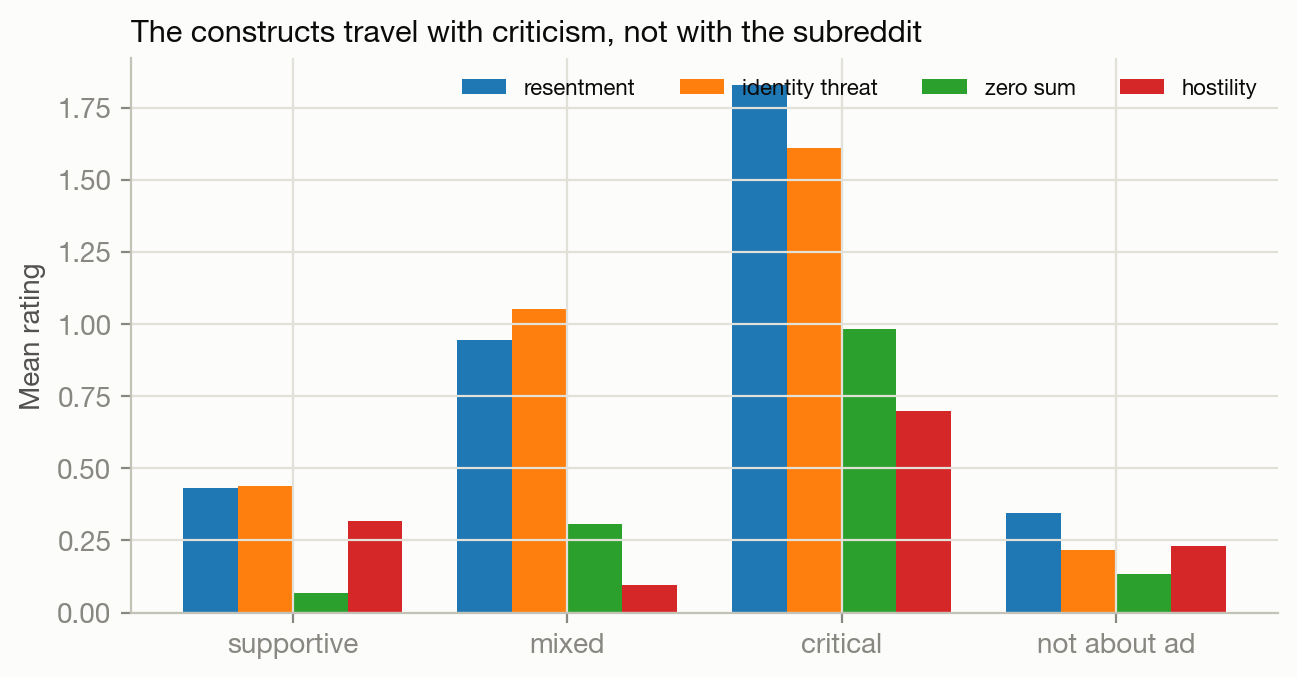
\includegraphics[width=0.88\linewidth]{figs/constructs_by_stance.png}
\caption{Constructs by coded stance}
\end{figure}

\section{Tone tells a different and weaker story}

Measured on tone alone, the two communities look alike: \textbf{both are strongly negative}, with
mean polarity $-0.335$ in r/MensLib and $-0.379$ in r/MensRights, and 53.8\,\% against 59.2\,\% of
comments read as negative. A reader expecting r/MensLib to have sounded positive about the
advertisement will not find that here.

\begin{figure}[h]
\centering
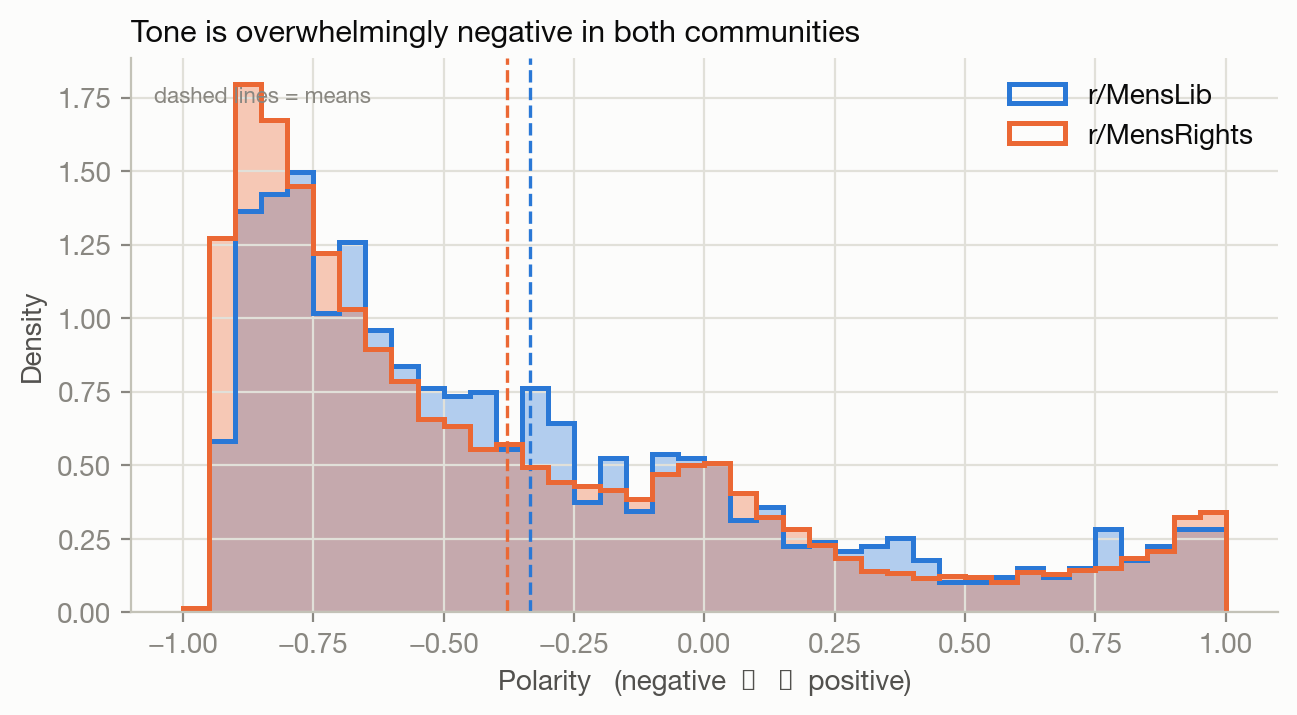
\includegraphics[width=0.92\linewidth]{figs/sentiment_distribution.png}
\caption{Polarity distributions; dashed lines are means}
\end{figure}

The distributions are bimodal in both communities, piling up at the negative end with a smaller
positive cluster and little in between. The difference between them is a modest shift in those
masses rather than a different shape.

\subsection*{Comment length hides most of the gap}

The raw tone difference is $+0.044$; adjusted for length it is $+0.123$. The reason is mechanical:
longer comments score more negative, falling from $-0.04$ in the shortest decile to about $-0.50$
in the longest, and r/MensLib comments are twice as long (median 50 words against 25). Within every
one of the ten length bands, r/MensLib is the less negative of the two.

\begin{figure}[h]
\centering
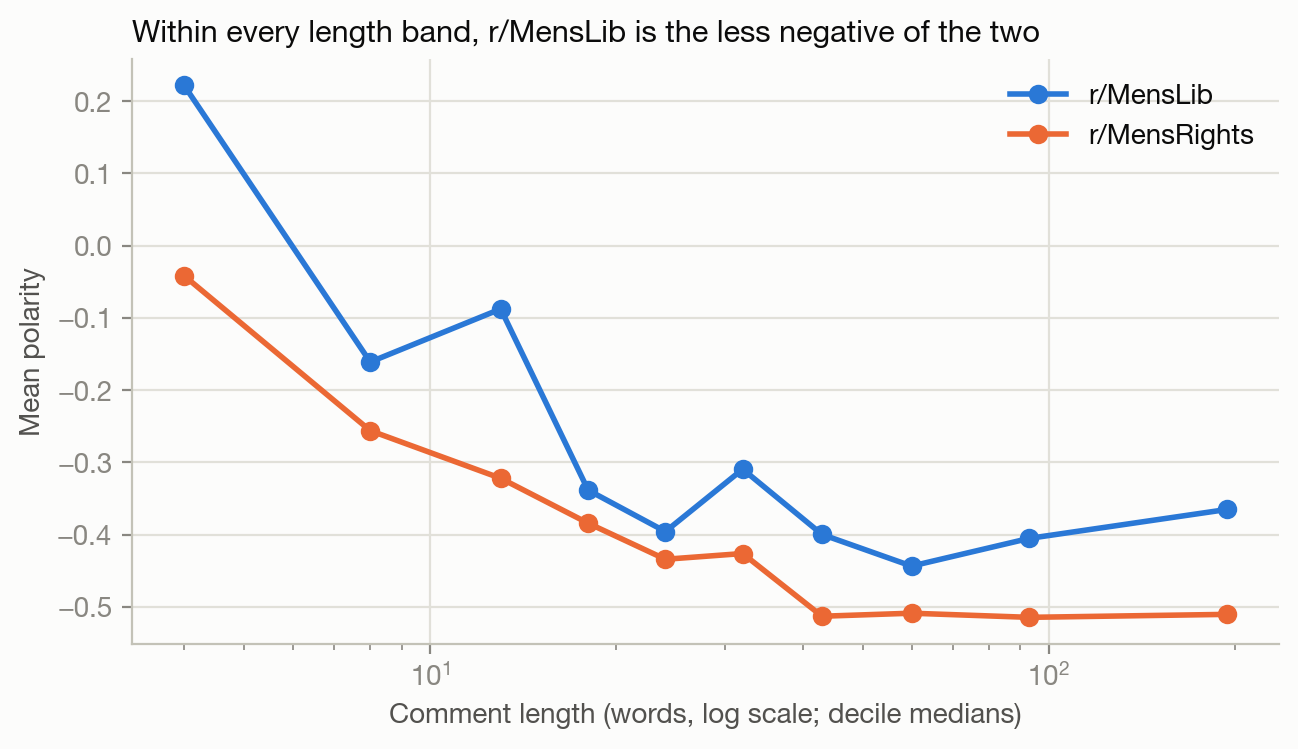
\includegraphics[width=0.88\linewidth]{figs/polarity_by_length.png}
\caption{Mean polarity by comment-length decile}
\end{figure}

In a bivariate regression the tone difference is statistically indistinguishable from zero
($p = 0.165$); once $\log$(words) enters, it is highly significant ($p = 1.3\times10^{-5}$). Any
tone comparison between communities with different writing norms needs this control, or it will
understate the difference.

\section{Why the tone result cannot carry weight, and the stance result can}

r/MensLib removed 22.4\,\% of its comments in these threads against r/MensRights' 4.9\,\%, and the
removed text is unrecoverable. This is selective attrition directly on the outcome, and it is the
reason the two results differ in standing.

\begin{figure}[h]
\centering
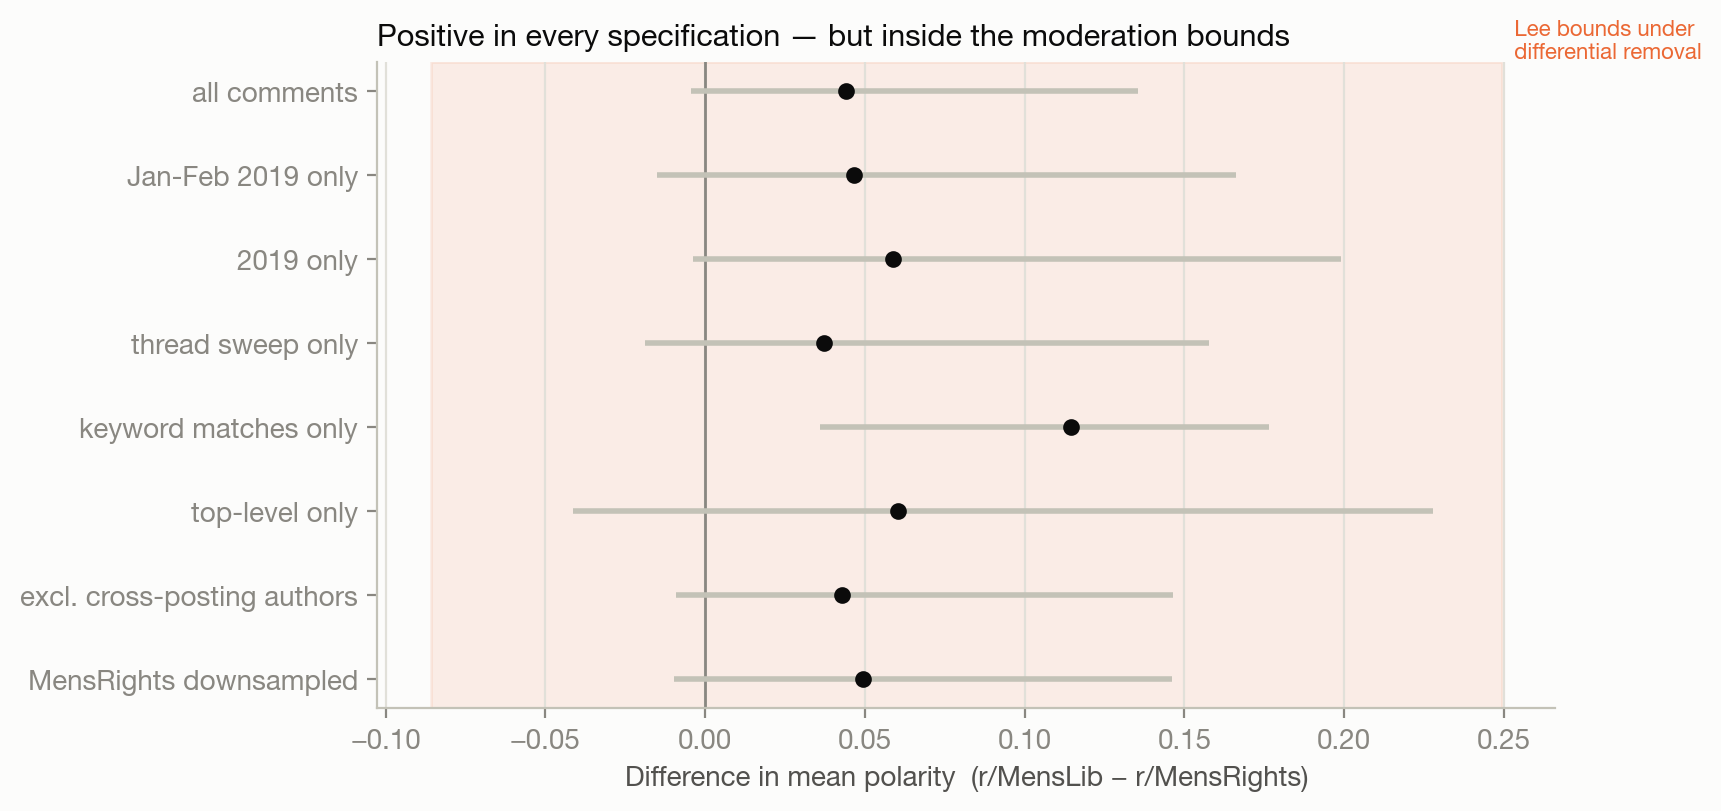
\includegraphics[width=0.92\linewidth]{figs/spec_curve.png}
\caption{Tone gap across specifications; the shaded band is the Lee bounds under differential
removal}
\end{figure}

For tone, bounds that account for the missing comments run from $-0.086$ to $+0.249$ and therefore
contain zero: the sign of the tone difference is \textbf{not identified}. Since moderation removes
hostile content, the naive estimate most likely flatters r/MensLib. For stance, the equivalent
worst-case bounds run from $-0.497$ to $-0.770$ and exclude zero, so the direction holds even under
the most adverse assumption. The stance comparison is the one that supports an inference.

\section{Emotional register and subject matter}

The emotional registers are near-identical. Anger sits at 0.155 in r/MensLib against 0.167 in
r/MensRights, and disgust at 0.204 against 0.203. The one real gap is \textbf{fear}, nearly twice
as present in r/MensLib (0.092 against 0.052), consistent with its comments discussing
vulnerability and what men are afraid to show; r/MensRights registers more surprise (0.084 against
0.060), the register of outrage and mockery.

\begin{figure}[h]
\centering
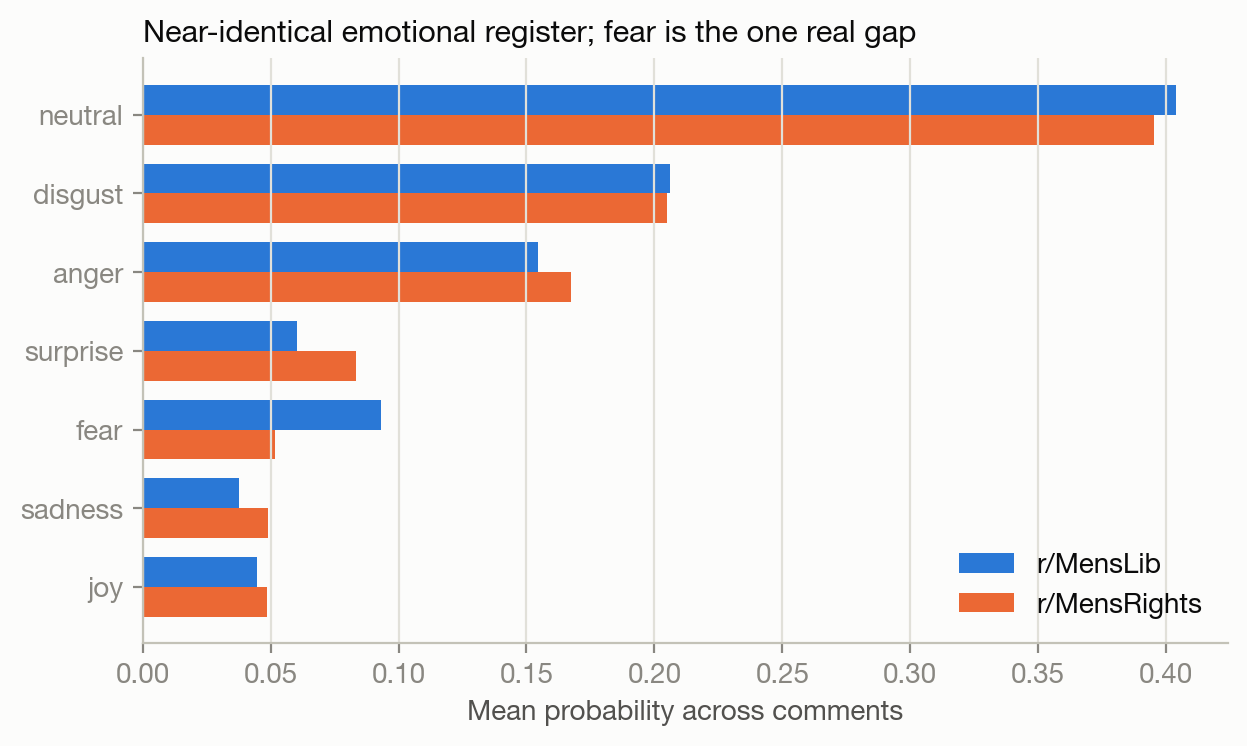
\includegraphics[width=0.88\linewidth]{figs/emotion_profile.png}
\caption{Mean emotion probability per comment}
\end{figure}

What separates the communities is subject matter. Clustering comments by meaning gives eight rough
groupings, and the division of attention is clear: r/MensLib argued \emph{inward} --- personal
testimony, and whether ``toxic masculinity'' is a useful term at all --- while r/MensRights argued
\emph{outward}, at feminism, at the brand, and at what to buy instead.

\begin{table}[h]
\centering\small
\caption{Theme prevalence, as a share of each community's comments}
\begin{tabular}{lccl}
\toprule
Theme & r/MensLib & r/MensRights & Skew \\
\midrule
Direct exchanges and personal experience & 33.2\,\% & 13.8\,\% & 2.4$\times$ r/MensLib \\
The term ``toxic masculinity''           & 11.7\,\% & 5.0\,\%  & 2.4$\times$ r/MensLib \\
Judging the advertisement itself         & 16.3\,\% & 9.8\,\%  & 1.7$\times$ r/MensLib \\
Feminism, patriarchy and gender politics & 14.2\,\% & 21.8\,\% & 1.5$\times$ r/MensRights \\
Gillette the brand and the backlash      & 6.5\,\%  & 12.7\,\% & 2.0$\times$ r/MensRights \\
Razors, shaving and products             & 3.0\,\%  & 8.9\,\%  & 3.0$\times$ r/MensRights \\
Corporate ethics, boycotts, other brands & 5.3\,\%  & 9.4\,\%  & 1.8$\times$ r/MensRights \\
Off-topic replies and one-liners         & 9.7\,\%  & 18.6\,\% & 1.9$\times$ r/MensRights \\
\bottomrule
\end{tabular}
\end{table}

\begin{figure}[h]
\centering
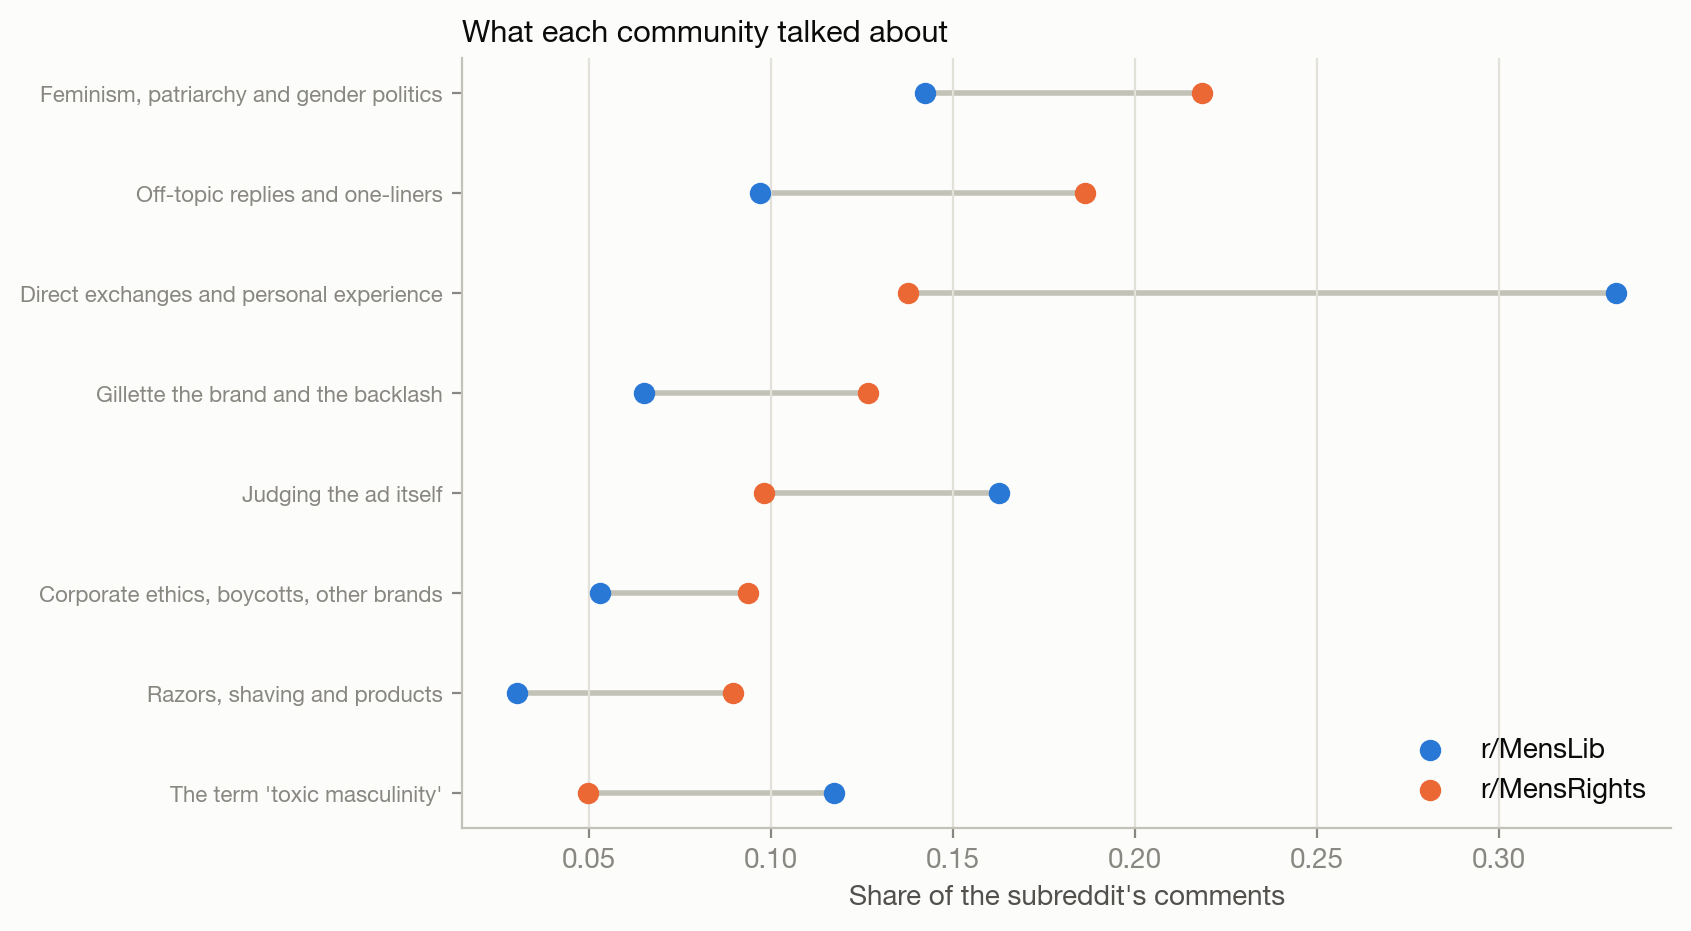
\includegraphics[width=0.88\linewidth]{figs/themes_dumbbell.png}
\caption{Theme prevalence by community}
\end{figure}

These clusters are soft groupings rather than recovered structure, and the labels are interpretive;
they should be read as a description of where attention went, not as a measurement.

\section{What these results do not establish}

\begin{enumerate}
\item \textbf{Stated position, not private belief.} The coding records the position a comment
takes, which need not be what its author holds.
\item \textbf{A narrow base on one side.} r/MensLib contributes 510 positioned comments across 58
threads, five of which hold 81\,\% of them. Its 71.8\,\% supportive share rests on a small number
of conversations.
\item \textbf{Conservative treatment of ambivalence.} ``Mixed'' is coded strictly, which may
understate genuine ambivalence in a forum like r/MensLib that rewards it.
\item \textbf{Unequal populations.} 4{,}846 r/MensRights authors against 549 in r/MensLib, with
time spans that diverge after 2019: r/MensLib effectively stopped discussing the advertisement
after that year, while r/MensRights continued to invoke it through 2026.
\end{enumerate}

\end{document}
